In questa sezione verranno elencati ed analizzati tutti i casi d'uso individuati dal gruppo. Ogni caso d'uso verrà identificato da un codice univoco secondo le regole descritte nel documento \textit{NormeDiProgetto\_v3.0.0} e riportate di seguito. 

\subsection{Denominazione dei casi d'uso}
Ad ogni caso d'uso saranno associate le seguenti informazioni:
\begin{itemize}
\item il codice del requisito che lo interessa UC-[Attore][Codice] dove Attore può essere:
	\begin{itemize}
		\item \textbf{G}: utente generico;
		\item \textbf{M}: moderatore;
		\item \textbf{S}: sviluppatore;
		\item \textbf{R}: utente riconosciuto;
		\item \textbf{N}: utente non riconosciuto;
		\item \textbf{I}: insegnante;
		\item \textbf{A}: allievo.
	\end{itemize}
\item un nome (univoco);
\item le pre-condizioni e le post-condizioni relative allo specifico caso d'uso;
\item gli attori coinvolti, sia primari che secondari;
\item lo scenario principale che il caso d'uso vorrebbe modellare;
\item le eventuali estensioni dello scenario principale.
\end{itemize}

\subsubsection{Gerarchie dei casi d'uso} 
Gli identificatori numerici assegnati a casi d'uso saranno organizzati gerarchicamente. Posto UC-[Attore]X codice di un caso d'uso, allora UC-[Attore]X.Y è sottocaso di UC-[Attore]X.

\subsection{Elenco dei casi d'uso - Utente generico}

	\subsubsection{UC-G1 Inserimento di una frase da svolgere}
	\begin{itemize}
		\item \textbf{Attori:} Utente generico.
		\item \textbf{Precondizione:} L'utente visualizza la vista principale dell'applicazione.
		\item \textbf{Postcondizione:} L'utente visualizza la vista per l'esecuzione dell'esercizio.
		\item \textbf{Scenario principale:}
		\begin{enumerate}
			\item l'utente scrive la frase da svolgere come esercizio
			\item l'utente conferma la frase indicata
		\end{enumerate}
	\end{itemize}

	\subsubsection{UC-G2 Selezione esercizio da svolgere}
	\begin{itemize}
			\item \textbf{Attori:} Utente generico.
			\item \textbf{Precondizione:} L'utente visualizza la lista degli esercizi ricercati.
			\item \textbf{Postcondizione:} L'utente visualizza la vista per l'esecuzione dell'esercizio.
			\item \textbf{Scenario principale:}
			\begin{enumerate}
					\item l'utente seleziona l'esercizio da svolgere
			\end{enumerate}
	\end{itemize}

	\subsubsection{UC-G3 Ricerca esercizi}
		\begin{itemize}
			\item\textbf{ Attori:} Utente generico.
			\item \textbf{Precondizione:} L'utente si trova nella vista principale dell'applicazione.
			\item \textbf{Postcondizione:} L'utente ottiene una lista degli esercizi filtrati.
			\item \textbf{Scenario principale:}
				\begin{enumerate}
					\item l'utente accede all'area dedicata alla ricerca degli esercizi
					\item l'utente scrive la frase o una sua parte nella barra di ricerca
					\item l'utente seleziona i filtri in base agli autori degli esercizi (UC-G3.1)
					\item l'utente seleziona i filtri in base alla difficoltà degli esercizi (UC-G3.2)
					\item l'utente seleziona i filtri in base agli argomenti degli esercizi (UC-G3.3)
					\item l'utente avvia la ricerca
					\item l'utente visualizza gli esercizi filtrati (UC-G3.4)
				\end{enumerate}
		\end{itemize}
%TODO: modifica diagramma
		\begin{figure}[h]
			\centering
			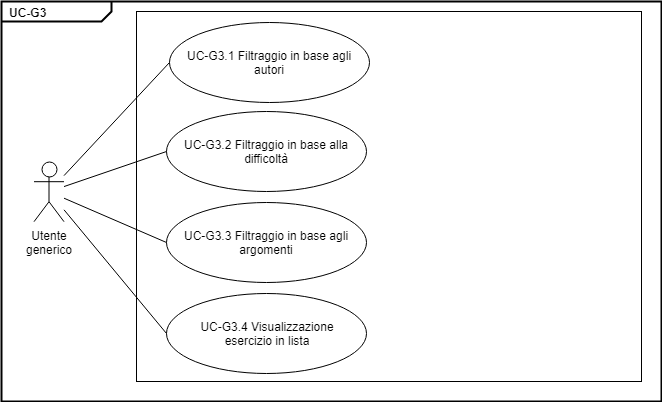
\includegraphics[scale=0.7]{images/UC-G3.png}
			\caption{UC-G3 Filtraggio esercizi}
		\end{figure}	

\subsubsection{UC-G3.1 Filtraggio in base agli autori}
	\begin{itemize}
		\item \textbf{Attori:} Utente generico.
		\item \textbf{Precondizione: } L'utente si trova nella vista di ricerca degli esercizi dell'applicazione.
		\item \textbf{Postcondizione: } L'utente ha indicato gli autori nel filtro di ricerca.
		\item \textbf{Scenario principale:}
		\begin{enumerate}
			\item l'utente visualizza la lista degli autori
			\item l'utente seleziona gli autori di cui vuole vedere gli esercizi
		\end{enumerate}
	\end{itemize}

\subsubsection{UC-G3.2 Filtraggio in base alla difficoltà}
	\begin{itemize}
		\item \textbf{Attori:} Utente generico.
		\item \textbf{Precondizione: } L'utente si trova nella vista di ricerca degli esercizi dell'applicazione.
		\item \textbf{Postcondizione: } L'utente ha indicato la difficoltà nel filtro di ricerca.
		\item \textbf{Scenario principale:}
		\begin{enumerate}
			\item l'utente visualizza i livelli possibili di difficoltà (da 1 a 5)
			\item l'utente indica il livello di difficoltà degli esercizi cercati
		\end{enumerate}
	\end{itemize}

	\subsubsection{UC-G3.3 Filtraggio in base agli argomenti}
		\begin{itemize}
			\item \textbf{Attori:} Utente generico.
			\item \textbf{Precondizione: } L'utente si trova nella vista di ricerca degli esercizi dell'applicazione.
			\item \textbf{Postcondizione: } L'utente ha indicato gli autori nel filtro di ricerca.
			\item \textbf{Scenario principale:}
			\begin{enumerate}
				\item l'utente visualizza la lista degli argomenti (pronomi, verbi, aggettivi, articoli, avverbi, ecc..)
				\item l'utente seleziona gli argomenti di cui vuole vedere gli esercizi
			\end{enumerate}
		\end{itemize}
		
\subsubsection{UC-G3.4 Visualizzazione esercizio in lista}
		\begin{itemize}
			\item \textbf{Attori:} Utente generico.
			\item \textbf{Precondizione: } L'utente si trova nella vista di ricerca degli esercizi dell'applicazione.
			\item \textbf{Postcondizione: } L'utente visualizza le informazioni di un esercizio.
			\item \textbf{Scenario principale:}
			\begin{enumerate}
				\item l'utente visualizza la frase inserita come esercizio
				\item l'utente visualizza la data di inserimento dell'esercizio
			\end{enumerate}
		\end{itemize}

	\subsubsection{UC-G4 Svolgimento esercizio}
		\begin{itemize}
			\item \textbf{Attori:} Utente generico.
			\item \textbf{Precondizione:}  L'utente visualizza la vista per l'esecuzione dell'esercizio.
			\item \textbf{Postcondizione:} L'utente visualizza la valutazione dell'esercizio.
			\item \textbf{Scenario principale:}
				\begin{enumerate}
					\item l'utente compila i campi (UC-G4.1).
					\item l'utente conferma i dati inseriti.
					\item l'utente visualizza la valutazione.
				\end{enumerate}
		\end{itemize}

	\subsubsection{UC-G4.1 Compilazione dei campi}
		\begin{itemize}
			\item \textbf{Attori:} Utente generico.
			\item \textbf{Precondizione:} L'utente ha selezionato un esercizio da eseguire.
			\item \textbf{Postcondizione:} L'utente ha compilato i campi proposti dall'esercizio.
			\item \textbf{Scenario principale:}
				\begin{enumerate}
					\item l'utente sceglie la classe grammaticale per ogni parola presentata
					\item l'utente conferma la soluzione dell'esercizio
				\end{enumerate}
		\end{itemize}
		
%TODO: inclusione in immagine e codice UC
	\subsubsection{UC-G5 Visualizzazione della valutazione dell'esercizio}
	\begin{itemize}
			\item \textbf{Attori:} Utente generico.
			\item \textbf{Precondizione:} L'utente ha completato l'esecuzione dell'esercizio.
			\item \textbf{Postcondizione:} L'allievo visualizza la valutazione dell'esercizio.
			\item \textbf{Scenario principale:}
				\begin{enumerate}
					\item l'allievo seleziona il correttore dell'esercizio (insegnante o algoritmo automatico)
					\item l'allievo visualizza la valutazione (da 1 a 10) in base al correttore scelto
				\end{enumerate}
	\end{itemize}				

\subsubsection{UC-G6 Segnalazione abuso di un esercizio}
	\begin{itemize}
		\item \textbf{Attori:} Utente generico.
		\item \textbf{Precondizione:} L'utente si trova nella vista di svolgimento di un esercizio che ritiene non conforme alle norme di comportamento.
		\item \textbf{Postcondizione:} L'utente ha inviato una notifica di abuso del codice di comportamento.
		\item \textbf{Scenario principale:}
		\begin{enumerate}
			\item l'utente seleziona l'opzione "Segnala abuso"
		\end{enumerate}
	\end{itemize}
	
	

\subsection{Elenco dei casi d'uso - Utente: Utente non riconosciuto}

\subsubsection{UC-N1 Visualizzazione pagina di registrazione}
	\begin{itemize}
		\item \textbf{Attori:} Utente non riconosciuto.
		\item \textbf{Precondizione:} L'utente si trova nella vista principale dell'applicazione.
		\item \textbf{Postcondizione:} L'utente si trova nella vista di registrazione dell'applicazione.
		\item \textbf{Scenario principale:}
		\begin{enumerate}
			\item l'utente seleziona l'opzione "Registrati"
		\end{enumerate}
	\end{itemize}


\subsubsection{UC-N2 Registrazione utente}
\begin{itemize}
		\item \textbf{Attori: }Utente non riconosciuto.
		\item \textbf{Precondizione: }L'utente si trova nella vista di registrazione dell'applicazione.
		\item \textbf{Postcondizione: }L'utente è registrato nel database locale.
		\item \textbf{Scenario principale: }
		\begin{enumerate}
		\item l'utente ha scelto di registrarsi al sistema, quindi di creare un nuovo profilo
		\item l'utente inserisce il proprio nome (UC-N2.1)
		\item l'utente inserisce il proprio cognome (UC-N2.2)
		\item l'utente inserisce l'username (UC-N2.3)
		\item l'utente inserisce la propria email (UC-N2.4)
		\item l'utente inserisce la password (UC-N2.5)
		\item l'utente fornirà il nome della scuola a cui appartiene (UC-N2.6)
		\item l'utente fornirà la città in cui si trova la scuola (UC-N2.7)
		\item l'utente indica il ruolo
		\item l'utente conferma la registrazione
		\end{enumerate}
		\item \textbf{Estensioni: }
		\begin{itemize}
			\item 10.a Nel caso in cui l'utente tenti l'inserimento di campi non validi vedrà comparire un messaggio d'errore "Campi non validi" (UC-N5).
		\end{itemize}
\end{itemize}

\begin{figure}[h]
	\centering
	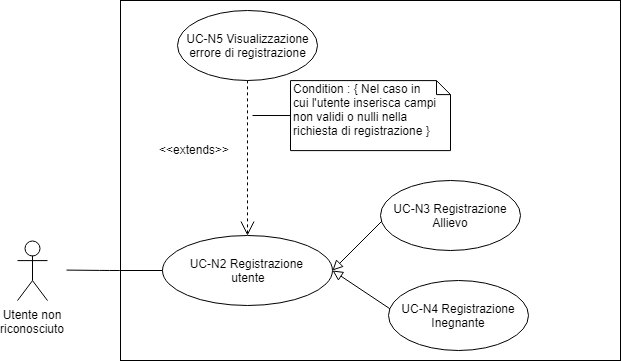
\includegraphics[scale=0.7]{images/UC-N2.png}
	\caption{UC-N2 Registrazione utente}
\end{figure}

\subsubsection{UC-N3 Registrazione Allievo}
\begin{itemize}
	\item \textbf{Attori: }Utente non riconosciuto.
	\item \textbf{Precondizione: }L'utente si trova nella vista di registrazione dell'applicazione.
	\item \textbf{Postcondizione: }L'utente è registrato nel database locale come allievo.
	\item \textbf{Scenario principale: }
		\begin{enumerate}
		\item l'utente ha scelto di registrarsi al sistema, quindi di creare un nuovo profilo
		\item l'utente inserisce il proprio nome (UC-N2.1)
		\item l'utente inserisce il proprio cognome (UC-1.2)
		\item l'utente inserisce l'username (UC-N2.3)
		\item l'utente inserisce la propria email (UC-N2.4)
		\item l'utente inserisce la password (UC-N2.5)
		\item l'utente fornirà il nome della scuola a cui appartiene (UC-N2.6)
		\item l'utente fornirà la città in cui si trova la scuola (UC-N2.7)
		\item l'utente indica come ruolo "Allievo"
		\item l'utente conferma la registrazione
		\end{enumerate}
\end{itemize}

\subsubsection{UC-N4 Registrazione Insegnante}
\begin{itemize}
	\item \textbf{Attori: }Utente non riconosciuto.
	\item \textbf{Precondizione: }L'utente si trova nella vista di registrazione dell'applicazione.
	\item \textbf{Postcondizione: }L'utente è registrato nel database locale ed in attesa di conferma.
	\item \textbf{Scenario principale: }
		\begin{enumerate}
		\item l'utente ha scelto di registrarsi al sistema, quindi di creare un nuovo profilo
		\item l'utente inserisce il proprio nome (UC-N2.1)
		\item l'utente inserisce il proprio cognome (UC-N2.2)
		\item l'utente inserisce l'username (UC-N2.3)
		\item l'utente inserisce la propria email (UC-N2.4)
		\item l'utente inserisce la password (UC-N2.5)
		\item l'utente fornirà il nome della scuola a cui appartiene (UC-N2.6)
		\item l'utente fornirà la città in cui si trova la scuola (UC-N2.7)
		\item l'utente indica come ruolo "Insegnante"
		\item l'utente inserisce il proprio codice INPS (UC-N4.1)
		\item l'utente conferma la registrazione
		\end{enumerate}
\end{itemize}

\subsubsection{UC-N4.1 Inserimento codice INPS}
\begin{itemize}
	\item \textbf{Attori: }Utente non riconosciuto.
	\item \textbf{Precondizione: }L'utente si trova nella vista di registrazione dell'applicazione e ha indicato l'iscrizione come insegnante.
	\item \textbf{Postcondizione: }
		L'utente ha inserito il codice INPS durante la procedura di registrazione come insegnante.
		\item \textbf{Scenario principale:}
		\begin{enumerate}
			\item l'utente inserisce il codice INPS nella cella dedicata
		\end{enumerate}
\end{itemize}

\subsubsection{UC-N2.1 Inserimento nome: registrazione}
\begin{itemize}
	\item \textbf{Attori: }Utente non riconosciuto.
	\item \textbf{Precondizione: }L'utente si trova nella vista 		di registrazione dell'applicazione.
	\item \textbf{Postcondizione: }L'utente ha inserito il nome durante la procedura di registrazione.
	\item \textbf{Scenario principale: }
	\begin{enumerate}
		\item l'utente inserisce il proprio nome nella cella 				dedicata
	\end{enumerate}
\end{itemize}

\subsubsection{UC-N2.2 Inserimento cognome: registrazione}
\begin{itemize}
	\item \textbf{Attori: }Utente non riconosciuto.
	\item \textbf{Precondizione: }L'utente si trova nella vista 		di registrazione dell'applicazione.
	\item \textbf{Postcondizione: }L'utente ha inserito il cognome durante la procedura di registrazione.
	\item \textbf{Scenario principale: }
	\begin{enumerate}
		\item l'utente inserisce il proprio cognome nella cella 				dedicata
	\end{enumerate}
\end{itemize}

\subsubsection{UC-N2.3 Inserimento username: registrazione}
\begin{itemize}
	\item \textbf{Attori: }Utente non riconosciuto.
	\item \textbf{Precondizione: }L'utente si trova nella vista 		di registrazione dell'applicazione.
	\item \textbf{Postcondizione: }L'utente ha inserito l'username durante la procedura di registrazione.
	\item \textbf{Scenario principale: }
	\begin{enumerate}
		\item l'utente inserisce il proprio username nella cella dedicata
	\end{enumerate}
\end{itemize}

\subsubsection{UC-N2.4 Inserimento email: registrazione}
\begin{itemize}
	\item \textbf{Attori: }Utente non riconosciuto.
	\item \textbf{Precondizione: }L'utente si trova nella vista 		di registrazione dell'applicazione.
	\item \textbf{Postcondizione: }L'utente ha inserito l'email durante la procedura di registrazione.
	\item \textbf{Scenario principale: }
	\begin{enumerate}
		\item l'utente inserisce la propria email nella cella dedicata
	\end{enumerate}
\end{itemize}

\subsubsection{UC-N2.5 Inserimento password: registrazione}
\begin{itemize}
	\item \textbf{Attori: }Utente non riconosciuto.
	\item \textbf{Precondizione: }L'utente si trova nella vista 		di registrazione dell'applicazione.
	\item \textbf{Postcondizione: }L'utente ha inserito la password durante la procedura di registrazione.
	\item \textbf{Scenario principale: }
	\begin{enumerate}
		\item l'utente inserisce la password nella cella dedicata
	\end{enumerate}
\end{itemize}

\subsubsection{UC-N2.6 Inserimento nome scuola: registrazione}
\begin{itemize}
	\item \textbf{Attori: }Utente non riconosciuto.
	\item \textbf{Precondizione: }L'utente si trova nella vista 		di registrazione dell'applicazione.
	\item \textbf{Postcondizione: }L'utente ha inserito il nome della scuola che frequenta durante la procedura di registrazione.
	\item \textbf{Scenario principale: }
	\begin{enumerate}
		\item l'utente inserisce il nome della scuola che frequenta nella cella dedicata
	\end{enumerate}
\end{itemize}

\subsubsection{UC-N2.7 Inserimento città: registrazione}
\begin{itemize}
	\item \textbf{Attori: }Utente non riconosciuto.
	\item \textbf{Precondizione: }L'utente si trova nella vista 		di registrazione dell'applicazione.
	\item \textbf{Postcondizione: }L'utente ha inserito la città a cui la scuola appartiene durante la procedura di registrazione.
	\item \textbf{Scenario principale: }
	\begin{enumerate}
		\item l'utente inserisce la città della scuola nella cella dedicata
	\end{enumerate}
\end{itemize}

\subsubsection{UC-N5 Visualizzazione errore di registrazione}
\begin{itemize}
	\item \textbf{Attori:} Utente non riconosciuto.
	\item \textbf{Precondizione:} L'utente ha confermato la richiesta di registrazione con campi non validi o nulli
	\item \textbf{Postcondizione:} L'utente torna alla vista di registrazione
	\item  \textbf{Scenario principale: }
	\begin{enumerate}
		\item visualizza un messaggio di errore "Registrazione non avvenuta: campi non validi"
	\end{enumerate}
\end{itemize}

\subsubsection{UC-N6 Autenticazione}
		\begin{itemize}
			\item \textbf{Attori:} Utente non riconosciuto.
			\item \textbf{Precondizione:} L'utente si trova nella vista di autenticazione dell'applicazione.
			\item \textbf{Postcondizione:} L'utente ha eseguito l'accesso con il proprio ruolo.
			\item \textbf{Scenario principale:}
				\begin{enumerate}
					\item l'utente inserisce il proprio username (UC-N6.1)
					\item l'utente inserisce la propria password (UC-N6.2)
					\item l'utente conferma l'accesso
				\end{enumerate}
				\item \textbf{Estensioni:}
				\begin{itemize}
					\item 2.a Nel caso in cui l'utente tenti l'inserimento di campi non validi vedrà comparire un messaggio d'errore (UC-N7).
				\end{itemize}
		\end{itemize}
	\begin{figure}[htbp]
			\centering
			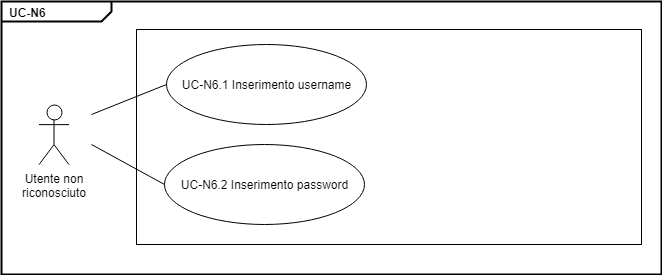
\includegraphics[scale=0.7]{images/UC-N6.png}
			\caption{UC-N6 Autenticazione}
		\end{figure}		
		
		

\subsubsection{UC-N6.1 Inserimento username: autenticazione}
\begin{itemize}
	\item \textbf{Attori:} Utente non riconosciuto.
			\item \textbf{Precondizione:} L'utente si trova nella vista di autenticazione dell'applicazione.
			\item \textbf{Postcondizione:} L'utente ha inserito il proprio username nella vista di autenticazione.
			\item \textbf{Scenario principale:}
				\begin{enumerate}
					\item l'utente scrive il proprio username nella cella apposita
				\end{enumerate}
\end{itemize}

\subsubsection{UC-N6.2 Inserimento password: autenticazione}
\begin{itemize}
	\item \textbf{Attori:} Utente non riconosciuto.
			\item \textbf{Precondizione:} L'utente si trova nella vista di autenticazione dell'applicazione.
			\item \textbf{Postcondizione:} L'utente ha inserito la propria password nella vista di autenticazione.
			\item \textbf{Scenario principale:}
				\begin{enumerate}
					\item l'utente scrive la propria password nella cella apposita
				\end{enumerate}
\end{itemize}
		
\subsubsection{UC-N7 Visualizzazione errore di autenticazione}
		\begin{itemize}
			\item \textbf{Attori:} Utente non riconosciuto.
			\item \textbf{Precondizione:} L'utente ha provato ad autenticarsi.
			\item \textbf{Postcondizione:} L'utente torna alla vista di accesso alla piattaforma.
			\item \textbf{Scenario principale:}
			\begin{enumerate}
				\item l'utente visualizza un messaggio di errore "Impossibile effettuare l'accesso: username o password errati"
			\end{enumerate}
		\end{itemize}
		
\subsection{Elenco dei casi d'uso - Utente: utente riconosciuto}
\subsubsection{UC-R1 Visualizzazione profilo personale}
\begin{itemize}
	\item \textbf{Attori:} Utente riconosciuto.
	\item \textbf{Precondizione:} L'utente si trova nella vista principale dell'applicazione.
	\item \textbf{Postcondizione:} L'utente si trova nella vista del proprio profilo.
	\item \textbf{Scenario principale:}
		\begin{enumerate}
			\item l'utente seleziona la voce "Profilo personale"
		\end{enumerate}
\end{itemize}

\subsubsection{UC-R2 Modifica profilo}
		\begin{itemize}
			\item \textbf{Attori:} Utente riconosciuto.
			\item \textbf{Precondizione:} L'utente si trova nella vista di modifica dei dati del proprio profilo.
			\item \textbf{Postcondizione:} L'utente ha modificato i propri dati personali.
			\item \textbf{Scenario principale:}
				\begin{enumerate}
					\item l'utente modifica l'username (UC-R2.1)
					\item  l'utente modifica la password (UC-R2.2)
					\item l'utente modifica la scuola che frequenta (UC-R2.3) 
					\item l'utente modifica la città a cui la scuola appartiene (UC-R2.4)
					\item l'utente conferma la modifica
				\end{enumerate}
				\item \textbf{Estensioni:}
				\begin{itemize}
					\item 2.a Nel caso in cui l'utente tenti l'inserimento di campi non validi vedrà comparire un messaggio d'errore (UC-R3).
				\end{itemize}
		\end{itemize}
		\begin{figure}[htbp]
			\centering
			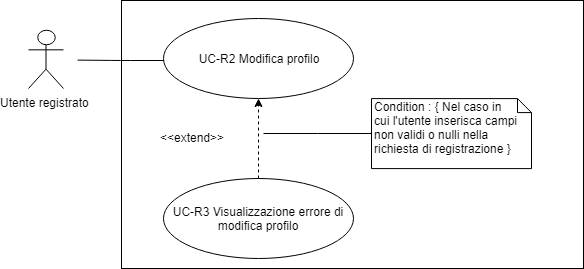
\includegraphics[scale=0.7]{images/UC-R2.png}
			\caption{UC-R2 Modifica profilo}
		\end{figure}
		
\subsubsection{UC-R2.1 Modifica username}
\begin{itemize}
			\item \textbf{Attori:} Utente riconosciuto.
			\item \textbf{Precondizione:} L'utente si trova nella vista di modifica dei dati del proprio profilo.
			\item \textbf{Postcondizione:} L'utente ha modificato il proprio username.
			\item \textbf{Scenario principale:}
			\begin{enumerate}
				\item l'utente inserisce il nuovo username nella cella apposita
			\end{enumerate}
\end{itemize}

\subsubsection{UC-R2.2 Modifica password}
\begin{itemize}
			\item \textbf{Attori:} Utente riconosciuto.
			\item \textbf{Precondizione:} L'utente si trova nella vista di modifica dei dati del proprio profilo.
			\item \textbf{Postcondizione:} L'utente ha modificato la propria password.
			\item \textbf{Scenario principale:}
			\begin{enumerate}
				\item l'utente inserisce la nuova password nella cella apposita
			\end{enumerate}
\end{itemize}

\subsubsection{UC-R2.3 Modifica scuola}
\begin{itemize}
			\item \textbf{Attori:} Utente riconosciuto.
			\item \textbf{Precondizione:} L'utente si trova nella vista di modifica dei dati del proprio profilo.
			\item \textbf{Postcondizione:} L'utente ha modificato la scuola a cui appartiene.
			\item \textbf{Scenario principale:}
			\begin{enumerate}
				\item l'utente inserisce la scuola a cui appartiene nella cella apposita
			\end{enumerate}
\end{itemize}

\subsubsection{UC-R2.4 Modifica città}
\begin{itemize}
			\item \textbf{Attori:} Utente riconosciuto.
			\item \textbf{Precondizione:} L'utente si trova nella vista di modifica dei dati del proprio profilo.
			\item \textbf{Postcondizione:} L'utente ha modificato la città a cui la scuola appartiene.
			\item \textbf{Scenario principale:}
			\begin{enumerate}
				\item l'utente inserisce la città a cui la scuola appartiene nella cella apposita
			\end{enumerate}
\end{itemize}

\subsubsection{UC-R3 Visualizzazione errore di modifica del profilo}	
	\begin{itemize}
		\item \textbf{Attori:} Utente riconosciuto.
		\item \textbf{Precondizione:} L'utente ha inserito dei campi non validi o nulli nella modifica del proprio profilo.
		\item \textbf{Postcondizione:} L'utente torna alla vista del proprio profilo.
		\item \textbf{Scenario principale:}
		\begin{enumerate}
			\item l'utente visualizza un messaggio di errore "Modifica del profilo non avvenuta: campi non validi o nulli"
		\end{enumerate}
	\end{itemize}

\subsubsection{UC-R4 Logout}
\begin{itemize}
		\item \textbf{Attori:} Utente riconosciuto.
		\item \textbf{Precondizione:} L'utente si trova in una qualsiasi vista dell'applicazione.
		\item \textbf{Postcondizione:} L'utente si è disconnesso dalla piattaforma.
		\item \textbf{Scenario principale:}
		\begin{enumerate}
			\item l'utente seleziona l'opzione "Logout"
		\end{enumerate}
	\end{itemize}

\subsection{Elenco dei casi d'uso - Utente: moderatore}	
\subsubsection{UC-M1 Verifica richiesta insegnante}
		\begin{itemize}
			\item \textbf{Attori:} Moderatore.
			\item \textbf{Precondizione:} Il moderatore si trova nella vista di amministrazione dell'applicazione.
			\item \textbf{Postcondizione:} Il moderatore ha confermato o rifiutato l'utente richiedente il ruolo di insegnante.
			\item \textbf{Scenario principale:}
				\begin{enumerate}
					\item il moderatore visualizza la lista contenente l'username degli utenti che richiedono il ruolo di insegnante (UC-M1.1)
					\item il moderatore seleziona un utente dalla lista
					\item il moderatore decide l'esito della richiesta (UC-M1.2)
				\end{enumerate}
		\end{itemize}	
		\begin{figure}[h]
		\centering
		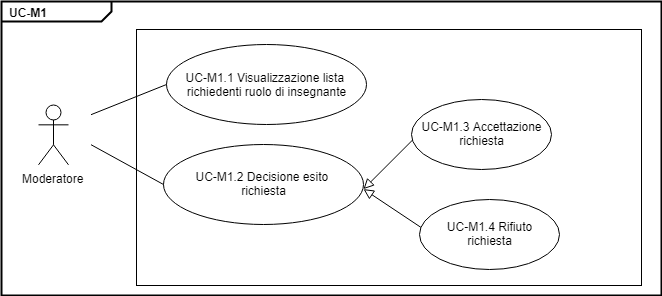
\includegraphics[scale=0.7]{images/UC-M1.png}
		\caption{UC-M1 Verifica richiesta insegnante}
	\end{figure}		
			
		
\subsubsection{UC-M1.1 Visualizzazione lista richiedenti ruolo insegnante}
	\begin{itemize}
		\item \textbf{Attori:} Moderatore.
		\item \textbf{Precondizione:} Il moderatore si trova nella vista di amministrazione dell'applicazione.
		\item \textbf{Postcondizione:} Il moderatore visualizza la lista di coloro che hanno fatto richiesta di registrazione come insegnante.
		\item \textbf{Scenario principale:}
			\begin{enumerate}
				\item il moderatore visualizza gli utenti che hanno fatto richiesta del ruolo insegnante (UC-M1.1.1)
			\end{enumerate}
	\end{itemize}
		
\subsubsection{UC-M1.1.1 Visualizzazione utenti richiedenti ruolo di insegnante}
	\begin{itemize}
		\item \textbf{Attori:} Moderatore.
		\item \textbf{Precondizione:} Il moderatore si trova nella vista di amministrazione dell'applicazione.
		\item \textbf{Postcondizione:} Il moderatore visualizza le credenziali di un richiedente del ruolo di insegnante.
		\item \textbf{Scenario principale:}
			\begin{enumerate}
				\item il moderatore visualizza nome del richiedente
				\item il moderatore visualizza cognome del richiedente
				\item il moderatore visualizza il codice INPS del richiedente
			\end{enumerate}
	\end{itemize}			

\subsubsection{UC-M1.2 Decisione esito richiesta}
	\begin{itemize}
		\item \textbf{Attori:} Moderatore.
		\item \textbf{Precondizione:} Il moderatore si trova nella vista di amministrazione dell'applicazione e ha selezionato un utente.
		\item \textbf{Postcondizione:} Il moderatore ha confermato o rifiutato l'utente richiedente il ruolo di insegnante.
		\item \textbf{Scenario principale:}
			\begin{enumerate}
				\item il moderatore conferma o rifiuta la richiesta
			\end{enumerate}
	\end{itemize}

\subsubsection{UC-M1.3 Accettazione richiesta}
	\begin{itemize}
		\item \textbf{Attori:} Moderatore.
		\item \textbf{Precondizione:} Il moderatore si trova nella vista di amministrazione dell'applicazione e ha selezionato un utente.
		\item \textbf{Postcondizione:} Il moderatore ha confermato l'utente richiedente il ruolo di insegnante.
		\item \textbf{Scenario principale:}
			\begin{enumerate}
				\item il moderatore conferma la richiesta
			\end{enumerate}
	\end{itemize}

\subsubsection{UC-M1.4 Rifiuto richiesta}
	\begin{itemize}
		\item \textbf{Attori:} Moderatore.
		\item \textbf{Precondizione:} Il moderatore si trova nella vista di amministrazione dell'applicazione e ha selezionato un utente.
		\item \textbf{Postcondizione:} Il moderatore ha rifiutato l'utente richiedente il ruolo di insegnante.
		\item \textbf{Scenario principale:}
			\begin{enumerate}
				\item il moderatore rifiuta la richiesta
			\end{enumerate}
	\end{itemize}

\subsubsection{UC-M2 Visualizzazione lista degli esercizi: moderatore}
	\begin{itemize}
		\item \textbf{Attori:} Moderatore.
		\item \textbf{Precondizione:} Il moderatore ha eseguito l'accesso all'area Esercizi e può aver svolto una ricerca tra gli esercizi.
		\item \textbf{Postcondizione:} Il moderatore visualizza una lista di esercizi inseriti nella piattaforma.
		\item \textbf{Scenario principale:}
			\begin{enumerate}
				\item il moderatore visualizza gli esercizi all'interno di una lista (UC-M2.1)
			\end{enumerate}
	\end{itemize}
		
\subsubsection{UC-M2.1 Visualizzazione esercizio inserito}
	\begin{itemize}
		\item \textbf{Attori:} Moderatore.
		\item \textbf{Precondizione:} Il moderatore ha eseguito l'accesso all'area Esercizi e può aver svolto una ricerca tra gli esercizi.
		\item \textbf{Postcondizione:} Il moderatore visualizza le informazioni di un esercizio presente nella piattaforma.
		\item \textbf{Scenario principale:}
			\begin{enumerate}
				\item il moderatore visualizza il codice associato all'esercizio
				\item il moderatore visualizza la frase dell'esercizio
				\item il moderatore visualizza l'username dell'autore dell'esercizio
				\item il moderatore visualizza la data in cui l'esercizio è stato inserito
			\end{enumerate}
	\end{itemize}		
		
\subsubsection{UC-M3 Ricerca esercizi: moderatore}
	\begin{itemize}
		\item \textbf{Attori:} Moderatore.
		\item \textbf{Precondizione:} Il moderatore ha effettuato l'accesso nell'area esercizi.
		\item \textbf{Postcondizione:} Il moderatore ottiene una lista degli esercizi contenenti la parola o le parole ricercate.
		\item \textbf{Scenario principale:}
			\begin{enumerate}
				\item il moderatore scrive nella barra di ricerca una frase o una sua parte
				\item il moderatore visualizza una lista di esercizi contenenti la parola o la frase cercata (UC-M2)
			\end{enumerate}
	\end{itemize}
	
	\begin{figure}[h]
		\centering
		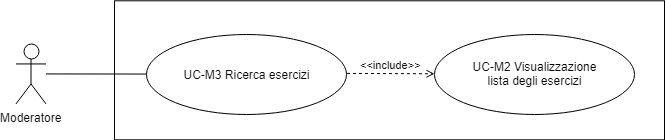
\includegraphics[scale=0.7]{images/UC-M3.png}
		\caption{UC-M3 Ricerca esercizi}
	\end{figure}	
	
\subsubsection{UC-M4 Eliminazione di un esercizio}
			\begin{itemize}
			\item \textbf{Attori:} Moderatore.
			\item \textbf{Precondizione:} Il moderatore visualizza la lista di esercizi.
			\item \textbf{Postcondizione:} Il moderatore ha eliminato l'esercizio desiderato.
			\item \textbf{Scenario principale:}
				\begin{enumerate}
					\item il moderatore indica gli esercizi da eliminare
					\item il moderatore conferma l'eliminazione dell'esercizio selezionato
				\end{enumerate}
		\end{itemize}

\subsubsection{UC-M5 Visualizzazione lista degli utenti: moderatore}
	\begin{itemize}
		\item \textbf{Attori:} Moderatore.
		\item \textbf{Precondizione:} Il moderatore ha eseguito l'accesso all'area Utenti e può aver svolto una ricerca tra gli utenti.
		\item \textbf{Postcondizione:} Il moderatore visualizza la lista degli utenti presenti nella piattaforma.
		\item \textbf{Scenario principale:}
			\begin{enumerate}
				\item il moderatore visualizza gli utenti presenti nella piattaforma (UC-M5.1)
			\end{enumerate}
	\end{itemize}
	
\subsubsection{UC-M5.1 Visualizzazione utente iscritto in lista}
	\begin{itemize}
		\item \textbf{Attori:} Moderatore.
		\item \textbf{Precondizione:} Il moderatore ha eseguito l'accesso all'area Utenti e può aver svolto una ricerca tra gli utenti.
		\item \textbf{Postcondizione:} Il moderatore visualizza le credenziali di un utente iscritto alla piattaforma.
		\item \textbf{Scenario principale:}
			\begin{enumerate}
				\item il moderatore visualizza il nome dell'utente
				\item il moderatore visualizza il cognome dell'utente
				\item il moderatore visualizza l'username di un utente
			\end{enumerate}
	\end{itemize}
		
\subsubsection{UC-M6 Ricerca utenti: moderatore}
	\begin{itemize}
		\item \textbf{Attori:} Moderatore.
		\item \textbf{Precondizione:} Il moderatore visualizza la lista degli utenti presenti nella piattaforma.
		\item \textbf{Postcondizione:} Il moderatore ottiene una lista degli utenti aventi nell'username la parola indicata.
		\item \textbf{Scenario principale:}
			\begin{enumerate}
				\item il moderatore scrive nella barra di ricerca una stringa
				\item il moderatore visualizza una lista di utenti il cui username contiene la stringa ricercata (UC-M5)
			\end{enumerate}
	\end{itemize}
	
	\begin{figure}[h]
		\centering
		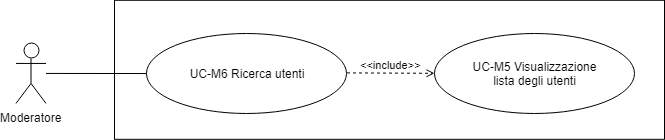
\includegraphics[scale=0.7]{images/UC-M6.png}
		\caption{UC-M6 Ricerca utenti}
	\end{figure}	

\subsubsection{UC-M7 Eliminazione di un utente}
\begin{itemize}
	\item \textbf{Attori:} Moderatore.
	\item \textbf{Precondizione:} Il moderatore visualizza la lista degli utenti.
	\item \textbf{Postcondizione:} Il moderatore ha eliminato l'utente desiderato.
	\item \textbf{Scenario principale:}
	\begin{enumerate}
		\item il moderatore indica uno o più utenti da eliminare
		\item il moderatore conferma l'eliminazione degli utenti selezionati
	\end{enumerate}
\end{itemize}

\subsubsection{UC-M8 Visualizzazione lista delle segnalazioni}
\begin{itemize}
	\item \textbf{Attori:} Moderatore.
	\item \textbf{Precondizione:} Il moderatore si trova nella vista di amministrazione dell'applicazione.
	\item \textbf{Postcondizione:} Il moderatore visualizza la lista delle segnalazioni ricevute.
	\item \textbf{Scenario principale:}
	\begin{enumerate}
		\item il moderatore seleziona l'opzione "Lista delle segnalazioni"
		\item il moderatore visualizza le segnalazioni effettuate (UC-M8.1)
	\end{enumerate}
\end{itemize}

\subsubsection{UC-M8.1 Visualizzazione segnalazione in lista}
\begin{itemize}
	\item \textbf{Attori:} Moderatore.
	\item \textbf{Precondizione:} Il moderatore si trova nella vista di amministrazione dell'applicazione.
	\item \textbf{Postcondizione:} Il moderatore visualizza le specifiche di una segnalazione.
	\item \textbf{Scenario principale:}
	\begin{enumerate}
		\item il moderatore visualizza la frase segnalata
		\item il moderatore visualizza la data della segnalazione
		\item il moderatore visualizza l'username dell'autore dell'esercizio segnalato
		\item il moderatore visualizza l'username dell'autore della segnalazione
	\end{enumerate}
\end{itemize}

\subsubsection{UC-M9 Eliminazione segnalazione}
\begin{itemize}
	\item \textbf{Attori:} Moderatore.
	\item \textbf{Precondizione:} Il moderatore visualizza la lista delle segnalazioni ricevute.
	\item \textbf{Postcondizione:} Il moderatore ha eliminato la segnalazione desiderata.
	\item \textbf{Scenario principale:}
	\begin{enumerate}
		\item Il moderatore seleziona la segnalazione
		\item Il moderatore seleziona l'opzione "Elimina segnalazione"
	\end{enumerate}
\end{itemize}

\subsubsection{UC-M10 Accesso all'area Esercizi}
\begin{itemize}
	\item \textbf{Attori:} Moderatore.
	\item \textbf{Precondizione:} Il moderatore si trova nell'area di amministrazione dell'applicazione.
	\item \textbf{Postcondizione:} Il moderatore ha eseguito l'accesso all'area esercizi.
	\item \textbf{Scenario principale:}
	\begin{enumerate}
		\item il moderatore seleziona l'opzione "Area esercizi"
		\item il moderatore visualizza la lista di tutti gli esercizi inseriti nella piattaforma (UC-M2)
	\end{enumerate}
\end{itemize}
\begin{figure}[h]
		\centering
		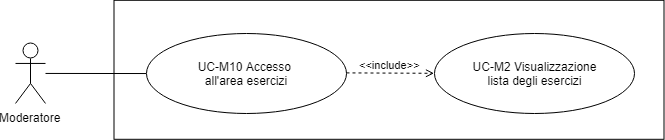
\includegraphics[scale=0.7]{images/UC-M10.png}
		\caption{UC-M10 Accesso all'area esercizi}
	\end{figure}	

\subsubsection{UC-M11 Accesso all'area Utenti}
\begin{itemize}
	\item \textbf{Attori:} Moderatore.
	\item \textbf{Precondizione:} Il moderatore si trova nell'area di amministrazione dell'applicazione.
	\item \textbf{Postcondizione:} Il moderatore ha eseguito l'accesso all'area utenti.
	\item \textbf{Scenario principale:}
	\begin{enumerate}
		\item il moderatore seleziona l'opzione "Area utenti"
		\item il moderatore visualizza la lista di tutti gli utenti iscritti alla piattaforma (UC-M5)
	\end{enumerate}
\end{itemize}

\begin{figure}[h]
		\centering
		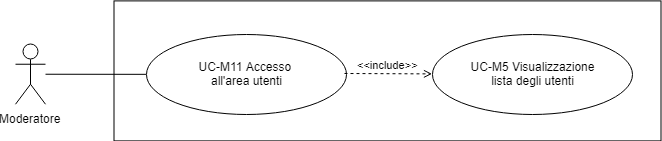
\includegraphics[scale=0.7]{images/UC-M11.png}
		\caption{UC-M11 Accesso all'area utenti}
	\end{figure}	

\subsection{Elenco dei casi d'uso - Utente: insegnante}		
\subsubsection{UC-I1 Visualizzazione lista esercizi inseriti}
\begin{itemize}
\item \textbf{Attori: }Insegnante.
		\item \textbf{Precondizione: }L'insegnante si trova nell'area Esercizi inseriti e può aver svolto una ricerca tra gli esercizi.
		\item \textbf{Postcondizione: }L'insegnante visualizza una lista di esercizi inseriti. 
		\item \textbf{Scenario principale:}
		\begin{enumerate}
			\item l'insegnante visualizza gli esercizi inseriti (UC-I1.1)
		\end{enumerate}
	\end{itemize}

\subsubsection{UC-I1.1 Visualizzazione esercizio inserito trovato}
\begin{itemize}
\item \textbf{Attori: }Insegnante.
		\item \textbf{Precondizione: }L'insegnante si trova nell'area Esercizi inseriti e può aver svolto una ricerca tra gli esercizi.
		\item \textbf{Postcondizione: }L'insegnante visualizza le specifiche di un esercizio inserito. 
		\item \textbf{Scenario principale:}
		\begin{enumerate}
			\item l'insegnante visualizza la frase dell'esercizio
			\item l'insegnante visualizza la data di inserimento dell'esercizio
		\end{enumerate}
	\end{itemize}

\subsubsection{UC-I2 Ricerca esercizi inseriti}
\begin{itemize}
	\item \textbf{Attori:} Insegnante.
	\item \textbf{Precondizione:} L'insegnante ha effettuato l'accesso all'area esercizi inseriti.
	\item \textbf{Postcondizione:} L'insegnante ottiene la lista degli esercizi contenenti la parola o le parole cercate.
	\item \textbf{Scenario principale:}
		\begin{enumerate}
				\item l'insegnante scrive nella barra di ricerca una frase o una sua parte
				\item l'insegnante visualizza una lista do esercizi contenenti la parola o la frase cercata (UC-I1)
		\end{enumerate}
\end{itemize}
\begin{figure}[h]
		\centering
		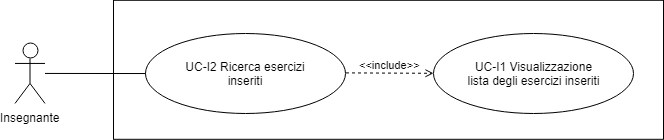
\includegraphics[scale=0.7]{images/UC-I2.png}
		\caption{UC-I2 Ricerca esercizi inseriti}
	\end{figure}	

\subsubsection{UC-I3 Modifica soluzione}
\begin{itemize}
	\item \textbf{Attori:} Insegnante.
	\item \textbf{Precondizione:} L'insegnante visualizza la lista degli esercizi inseriti.
	\item \textbf{Postcondizione:} La soluzione inserita è stata modificata.
	\item \textbf{Scenario principale:}
		\begin{enumerate}
		\item l'insegnante visualizza le parole della frase associate alle classi grammaticali indicati nella precedente soluzione
		\item l'insegnante modifica le classi grammaticali associate alle parole dell'esercizio
		\item l'insegnante conferma la modifica
		\end{enumerate}
\end{itemize}
	
\subsubsection{UC-I4 Eliminare una soluzione di un esercizio}
\begin{itemize}
	\item \textbf{Attori:} Insegnante.
	\item \textbf{Precondizione:} L'insegnante visualizza la lista degli esercizi inseriti.
	\item \textbf{Postcondizione:} Le soluzioni selezionate vengono eliminate.
	\item \textbf{Scenario principale:}
		\begin{enumerate}
			\item l'insegnante seleziona una o più soluzioni da eliminare
			\item l'insegnante conferma l'eliminazione
		\end{enumerate}
\end{itemize}

\subsubsection{UC-I5 Visualizzazione area di inserimento nuovo esercizio}
\begin{itemize}
		\item \textbf{Attori: }Insegnante.
		\item \textbf{Precondizione: }L'insegnante è nella vista principale dell'applicazione.
		\item \textbf{Postcondizione: }L'insegnante è nella vista di inserimento di un nuovo esercizio.
		\item \textbf{Scenario principale: }
	\begin{enumerate} 
		\item l'insegnante seleziona la voce "Inserisci esercizio"
	\end{enumerate}
\end{itemize}

\subsubsection{UC-I6 Inserimento esercizio}
	\begin{itemize}
		\item \textbf{Attori: }Insegnante.
		\item \textbf{Precondizione: }L'insegnante è nella vista di inserimento di un nuovo esercizio.
		\item \textbf{Postcondizione: }L'esercizio è stato inserito.
		\item \textbf{Scenario principale: }
			\begin{enumerate} 
				\item l'insegnante inserisce la frase
				\item l'insegnante inserisce la soluzione (UC-I6.1)
				\item l'insegnante inserisce gli argomenti (UC-I6.2)
				\item l'insegnante inserisce la difficoltà (UC-I6.3)
				\item l'insegnante conferma l'inserimento
			\end{enumerate}
		\item \textbf{Estensioni:} 
			\begin{itemize}
				\item 1.a Nel caso in cui la frase inserita sia nulla, viene visualizzato un errore (UC-I7)
			\end{itemize}
	\end{itemize}
	\begin{figure}[h]
		\centering
		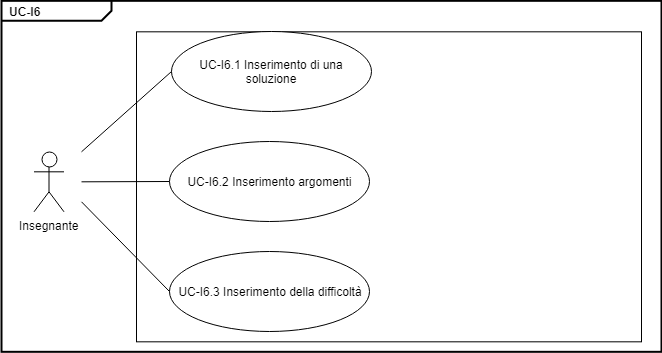
\includegraphics[scale=0.7]{images/UC-I6.png}
		\caption{UC-I6 Inserimento esercizio}
	\end{figure}

\subsubsection{UC-I6.1 Inserimento di una soluzione}
\begin{itemize}
\item \textbf{Attori: }Insegnante.
\item \textbf{Precondizione: }L'insegnante è nella vista di inserimento di un nuovo esercizio.
\item \textbf{Postcondizione: }L'insegnante ha inserito la propria soluzione.
\item \textbf{Scenario principale: }
		\begin{enumerate} 
		\item l'insegnante visualizza la soluzione proposta dal generatore automatico
		\item l'insegnante può modificare le classi grammaticali assegnate dal generatore automatico che ritiene errate
		\item l'insegnante seleziona lo stato della soluzione inserita, pubblica o privata
		\item l'insegnante conferma la soluzione
		\end{enumerate}	
\end{itemize}

\subsubsection{UC-I6.2 Inserimento argomenti}
\begin{itemize}
\item \textbf{Attori: }Insegnante.

\item \textbf{Precondizione:} L'insegnante sta inserendo un esercizio, gli viene richiesta la compilazione di una lista di argomenti presenti nell'esercizio.
\item \textbf{Postcondizione:} L'insegnante ha selezionato gli argomenti trattati nell'esercizio.
\item \textbf{Scenario principale: }
		\begin{enumerate}
		\item l'insegnante visualizza la lista degli argomenti
		\item l'insegnante seleziona gli argomenti che vengono toccati nell'esercizio
		\end{enumerate}
\end{itemize}				

\subsubsection{UC-I6.3 Inserimento della difficoltà}
\begin{itemize}
	\item \textbf{Attori: }Insegnante.
	\item \textbf{Precondizione:} L'insegnante è nella vista di inserimento di un nuovo esercizio.
	\item \textbf{Postcondizione:} L'insegnante ha indicato il livello di difficoltà.
	\item \textbf{Scenario principale:}
	\begin{enumerate}
		\item l'insegnante visualizza i livelli possibili di difficoltà (da 1 a 5)
		\item l'insegnante indica il livello di difficoltà dell'esercizio da inserire
	\end{enumerate}
\end{itemize}

\subsubsection{UC-I7 Visualizzazione errore di inserimento di una frase vuota}
\begin{itemize}
	\item \textbf{Attori:} Insegnante.
	\item \textbf{Precondizione:} L'insegnante è nella vista di inserimento di un nuovo esercizio e ha inserito una frase vuota.
	\item \textbf{Postcondizione:} L'insegnante torna alla vista di inserimento dell'esercizio.
	\item \textbf{Scenario principale:}
	\begin{enumerate}
		\item l'insegnante visualizza un messaggio di errore "La frase inserita è vuota"
	\end{enumerate}
\end{itemize}

\subsubsection{UC-I8 Creazione di una classe}
\begin{itemize}
	\item \textbf{Attori:} Insegnante.
	\item \textbf{Precondizione:} L'insegnante si trova nella vista del proprio profilo.
	\item \textbf{Postcondizione:} L'insegnante si trova nella vista di gestione della classe creata.
	\item \textbf{Scenario principale:}
	\begin{enumerate}
		\item l'insegnante selezione l'opzione "Crea classe"
		\item l'insegnante inserisce il nome della classe (UC-I8.1)
		\item l'insegnante inserisce la descrizione della classe (UC-I8.2)
		\item l'insegnante conferma la creazione
	\end{enumerate}
\end{itemize}

\begin{figure}[h]
		\centering
		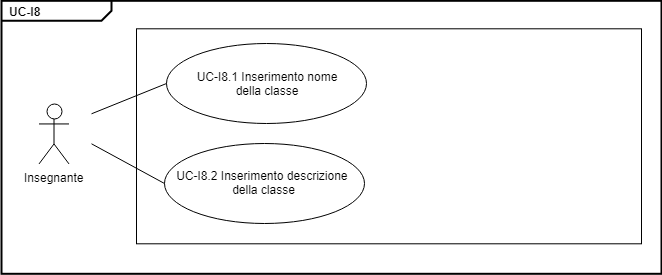
\includegraphics[scale=0.7]{images/UC-I8.png}
		\caption{UC-I8 Creazione di una classe}
	\end{figure}

\subsubsection{UC-I8.1 Inserimento nome della classe}
\begin{itemize}
	\item \textbf{Attori:} Insegnante.
	\item \textbf{Precondizione:} L'insegnante si trova nella vista del proprio profilo e ha selezionato la creazione di una nuova classe.
	\item \textbf{Postcondizione:} L'insegnante ha inserito il nome della classe durante la creazione della classe.
	\item \textbf{Scenario principale:}
	\begin{enumerate}
		\item l'insegnante inserisce il nome della classe nella cella appropriata
	\end{enumerate}
\end{itemize}

\subsubsection{UC-I8.2 Inserimento desrizione della classe}
\begin{itemize}
	\item \textbf{Attori:} Insegnante.
	\item \textbf{Precondizione:} L'insegnante si trova nella vista del proprio profilo e ha selezionato la creazione di una nuova classe.
	\item \textbf{Postcondizione:} L'insegnante ha inserito la descrizione della classe durante la creazione della classe.
	\item \textbf{Scenario principale:}
	\begin{enumerate}
		\item l'insegnante inserisce la descrizione della classe nella cella appropriata
	\end{enumerate}
\end{itemize}

\subsubsection{UC-I9 Eliminazione di una classe}
\begin{itemize}
	\item \textbf{Attori:} Insegnante.
	\item \textbf{Precondizione:} L'insegnante si trova nella vista di gestione di una propria classe.
	\item \textbf{Postcondizione:} L'insegnante elimina la classe dal sistema.
	\item \textbf{Scenario principale:}
	\begin{enumerate}
		\item l'insegnante clicca sul pulsante di eliminazione della classe
		\item l'insegnante conferma l'eliminazione
	\end{enumerate}
\end{itemize}

\subsubsection{UC-I10 Inserimento alunni}
\begin{itemize}
	\item \textbf{Attori:} Insegnante.
	\item \textbf{Precondizione:} L'insegnante si trova nella vista di gestione di una propria classe.
	\item \textbf{Postcondizione:} L'insegnante visualizza gli alunni inseriti.
	\item \textbf{Scenario principale:}
	\begin{enumerate}
		\item l'insegnante seleziona l'opzione "Aggiungi alunni"
		\item l'insegnante indica gli studenti da aggiungere (UC-I10.1)
		\item l'insegnante conferma l'inserimento
	\end{enumerate}
\end{itemize}

\subsubsection{UC-I10.1 Selezione alunni per l'inserimento}
\begin{itemize}
	\item \textbf{Attori:} Insegnante.
	\item \textbf{Precondizione:} l'insegnante si trova nella vista di aggiunta degli alunni a una classe
	\item \textbf{Postcondizione:} l'insegnante ha indicato gli alunni da inserire nella classe
	\item \textbf{Scenario principale:}
	\begin{enumerate}
		\item l'insegnante visualizza la lista di tutti gli alunni presenti sulla piattaforma (UC-I10.1.1)
		\item l'insegnante ricerca gli alunni da inserire (UC-I10.1.2)	
		\item l'insegnante seleziona gli alunni da inserire
	\end{enumerate}
\end{itemize}

\begin{figure}[h]
		\centering
		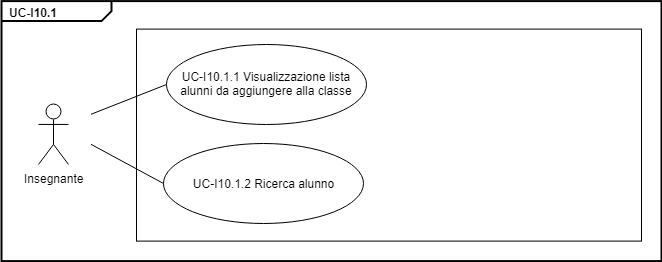
\includegraphics[scale=0.7]{images/UC-I10_1.png}
		\caption{UC-I10.1 Selezione alunni per l'inserimento}
	\end{figure}

\subsubsection{UC-I10.1.1 Visualizzazione lista alunni da aggiungere alla classe}
\begin{itemize}
	\item \textbf{Attori:} Insegnante.
	\item \textbf{Precondizione:} l'insegnante si trova nella vista di aggiunta degli alunni a una classe
	\item \textbf{Postcondizione:} l'insegnante visualizza la lista di tutti gli alunni presenti sulla piattaforma.
	\item \textbf{Scenario principale:}
	\begin{enumerate}
		\item l'insegnante visualizza gli alunni iscritti alla piattaforma (UC-I10.1.1.1)
	\end{enumerate}
\end{itemize}

\subsubsection{UC-I10.1.1.1 Visualizzazione alunno da aggiungere alla classe}
\begin{itemize}
	\item \textbf{Attori:} Insegnante.
	\item \textbf{Precondizione:} l'insegnante si trova nella vista di aggiunta degli alunni a una classe
	\item \textbf{Precondizione:} l'insegnante visualizza le credenziali di un alunno da aggiungere in una classe.
	\item \textbf{Scenario principale:}
	\begin{enumerate}
		\item l'insegnante visualizza il nome dell'alunno
		\item l'insegnante visualizza il cognome dell'alunno
		\item l'insegnante visualizza l'username dell'alunno
	\end{enumerate}
\end{itemize}

\subsubsection{UC-I10.1.2 Ricerca alunno}
\begin{itemize}
	\item \textbf{Attori:} Insegnante.
	\item \textbf{Precondizione:} L'insegnante visualizza la lista di tutti gli alunni presenti sulla piattaforma.
	\item \textbf{Postcondizione:} L'insegnante visualizza una lista di username contenenti la stringa inserita.
	\item \textbf{Scenario principale:}
	\begin{enumerate}
		\item l'insegnante scrive l'username di un alunno, o una sua parte
	\end{enumerate}
\end{itemize}

\subsubsection{UC-I11 Assegnazione esercizi}
\begin{itemize}
	\item \textbf{Attori:} Insegnante.
	\item \textbf{Precondizione:} Visualizza una lista di esercizi da una ricerca eseguita.
	\item \textbf{Postcondizione:} L'insegnante ha assegnato esercizi alla classe.
	\item \textbf{Scenario principale:}
	\begin{enumerate}
		\item l'insegnante seleziona degli esercizi in lista da assegnare
		\item l'insegnante indica la classe a cui assegnarli
		\item l'insegnante conferma l'assegnazione
	\end{enumerate}
\end{itemize}

\subsubsection{UC-I12 Visualizzazione lista delle classi}		
\begin{itemize}
	\item \textbf{Attori:} Insegnante.
	\item \textbf{Precondizione:} L'insegnante si trova nella vista del proprio profilo.
	\item \textbf{Postcondizione:} L'insegnante visualizza la lista delle classi create.
	\item \textbf{Scenario principale:}
	\begin{enumerate}
		\item l'insegnante seleziona l'opzione "vedi classi"
		\item l'insegnante visualizza le classi create (UC-I12.1)
	\end{enumerate}		
\end{itemize}

\subsubsection{UC-I12.1 Visualizzazione classe in lista}		
\begin{itemize}
	\item \textbf{Attori:} Insegnante.
	\item \textbf{Precondizione:} L'insegnante si trova nella vista del proprio profilo.
	\item \textbf{Postcondizione:} L'insegnante visualizza le informazioni riguardanti una classe.
	\item \textbf{Scenario principale:}
	\begin{enumerate}
		\item l'insegnante visualizza il nome della classe creata
		\item l'insegnante visualizza la descrizione della classe creata
		\item l'insegnante visualizza la data di creazione della classe
		\item l'insegnante visualizza il numero di alunni iscritti alla classe
	\end{enumerate}		
\end{itemize}

\subsubsection{UC-I13 Visualizzazione area di gestione di una classe}
\begin{itemize}
	\item \textbf{Attori:} Insegnante.
	\item \textbf{Precondizione:} L'insegnante visualizza la lista delle classi create.
	\item \textbf{Postcondizione:} L'insegnante visualizza la vista di gestione di una propria classe.
	\item \textbf{Scenario principale:}
	\begin{enumerate}
		\item l'insegnante seleziona una classe
	\end{enumerate}
\end{itemize}

\subsubsection{UC-I14 Visualizzazione lista degli alunni iscritti alla classe}		
\begin{itemize}
	\item \textbf{Attori:} Insegnante.
	\item \textbf{Precondizione:} L'insegnante si trova nella vista di gestione di una propria classe.
	\item \textbf{Postcondizione:} L'insegnante visualizza l'elenco degli alunni iscritti.
	\item \textbf{Scenario principale:}
	\begin{enumerate}
		\item l'insegnante seleziona l'opzione "vedi alunni"
		\item l'insegnante visualizza gli alunni iscritti alla classe (UC-I14.1)
			\end{enumerate}		
\end{itemize}

\subsubsection{UC-I14.1 Visualizzazione alunno iscritto alla classe in lista}		
\begin{itemize}
	\item \textbf{Attori:} Insegnante.
	\item \textbf{Precondizione:} L'insegnante si trova nella vista di gestione di una propria classe.
	\item \textbf{Postcondizione:} L'insegnante visualizza le credenziali di un alunno iscritto alla classe.
	\item \textbf{Scenario principale:}
	\begin{enumerate}
		\item l'insegnante visualizza il nome dell'alunno iscritto alla classe
		\item l'insegnante visualizza il cognome dell'alunno iscritto alla classe
		\item l'insegnante visualizza l'username dell'alunno iscritto alla classe
			\end{enumerate}		
\end{itemize}

\subsubsection{UC-I15 Visualizzare i progressi di un alunno della classe}
\begin{itemize}
	\item \textbf{Attori:} Insegnante.
	\item \textbf{Precondizione}: L'insegnante visualizza la lista degli alunni iscritti alla classe.
	\item \textbf{Postcondizione:} L'insegnante visualizza i progressi relativi allo studente selezionato.
	\item \textbf{Scenario principale:}
	\begin{enumerate}
		\item l'insegnante seleziona uno studente
		\item l'insegnante visualizza i grafici che riportano la media totale, la media per tipologia di esercizi e lo sviluppo della media nel tempo
	\end{enumerate}
\end{itemize}

\subsubsection{UC-I16 Elimina alunno dalla classe}		
\begin{itemize}
	\item \textbf{Attori:} Insegnante.
	\item \textbf{Precondizione:} L'insegnante visualizza la lista degli alunni della classe.
	\item \textbf{Postcondizione:} L'insegnante ha rimosso l'allievo dalla classe.
	\item \textbf{Scenario principale:}
	\begin{enumerate}
		\item l'insegnante seleziona l'allievo da rimuovere dalla classe
		\item l'insegnante conferma l'eliminazione
	\end{enumerate}	
\end{itemize}

\subsubsection{UC-I17 Accesso all'area Esercizi inseriti}		
\begin{itemize}
	\item \textbf{Attori:} Insegnante.
	\item \textbf{Precondizione:} L'insegnante si trova nell'area del proprio profilo personale.
	\item \textbf{Postcondizione:} L'insegnante ha eseguito l'accesso all'area esercizi inseriti.
	\item \textbf{Scenario principale:}
	\begin{enumerate}
		\item l'insegnante seleziona l'opzione "Area esercizi inseriti"
		\item l'insegnante visualizza la lista di tutti gli esercizi da lei inseriti (UC-I1)
	\end{enumerate}	
\end{itemize}
\begin{figure}[h]
		\centering
		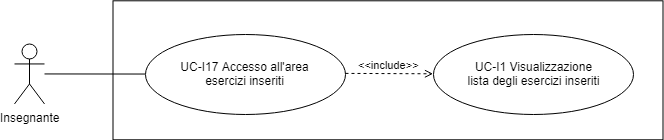
\includegraphics[scale=0.7]{images/UC-I17.png}
		\caption{UC-I17 Accesso all'area esercizi inseriti}
	\end{figure}	

\subsection{Elenco dei casi d'uso - Utente: allievo}
	\subsubsection{UC-A1 Visualizzazione progressi}
	\begin{itemize}
			\item \textbf{Attori:} Allievo.
			\item \textbf{Precondizione:} L'allievo si trova nella vista del proprio profilo.
			\item \textbf{Postcondizione:} L'allievo visualizza i progressi svolti fino a quel momento.
			\item \textbf{Scenario principale:}
				\begin{enumerate}
					\item L'allievo visualizza la media delle valutazioni ricevute, la media per tipologia di esercizi e lo sviluppo della media nel tempo
				\end{enumerate}
	\end{itemize}
	
	\subsubsection{UC-A2 Visualizzazione lista delle classi di appartenenza}
		\begin{itemize}
			\item \textbf{Attori:} Allievo.
			\item \textbf{Precondizione:} L'allievo si trova nella vista del proprio profilo.
			\item \textbf{Postcondizione:} L'allievo visualizza la lista delle classi a cui appartiene.
			\item \textbf{Scenario principale:}
			\begin{enumerate}
				\item l'allievo seleziona l'opzione "Lista delle classi"
				\item l'allievo visualizza le classi a cui appartiene
			\end{enumerate}
		\end{itemize}			

\subsubsection{UC-A2.1 Visualizzazione classe di appartenenza in lista}
		\begin{itemize}
			\item \textbf{Attori:} Allievo.
			\item \textbf{Precondizione:} L'allievo si trova nella vista del proprio profilo.
			\item \textbf{Postcondizione:} L'allievo visualizza le informazioni di una classe a cui appartiene.
			\item \textbf{Scenario principale:}
			\begin{enumerate}
				\item L'allievo visualizza il nome della classe
				\item L'allievo visualizza il nome dell'insegnante creatore della classe
				\item L'allievo visualizza il cognome dell'insegnante creatore della classe
				\item L'allievo visualizza la descrizione della classe
			\end{enumerate}
		\end{itemize}	

	\subsubsection{UC-A3 Annullamento dell'iscrizione a una classe}
		\begin{itemize}
			\item \textbf{Attori:} Allievo.
			\item \textbf{Precondizione:} L'allievo visualizza la lista delle classi a cui appartiene.
			\item \textbf{Postcondizione:} L'allievo ha annullato l'iscrizione alla classe.
			\item \textbf{Scenario principale:}
			\begin{enumerate}
				\item l'allievo seleziona l'opzione "Disiscriviti" in corrispondenza di una classe
			\end{enumerate}
		\end{itemize}					
				
	\subsubsection{UC-A4 Visualizzazione delle informazioni della classe}
		\begin{itemize}
			\item \textbf{Attori:} Allievo.
			\item \textbf{Precondizione:} L'allievo visualizza la lista delle classi a cui appartiene.
			\item \textbf{Postcondizione:} L'allievo visualizza le informazioni della classe indicata (allievi iscritti, media delle valutazioni ed esercizi assegnati).
			\item \textbf{Scenario principale:}
			\begin{enumerate}
				\item l'allievo seleziona una classe
			\end{enumerate}
		\end{itemize}
		
\subsubsection{UC-A5 Seleziona esercizio assegnato}
\begin{itemize}
			\item \textbf{Attori:} Allievo.
			\item \textbf{Precondizione:} L'allievo visualizza le informazioni della classe indicata (allievi iscritti, media delle valutazioni ed esercizi assegnati).
			\item \textbf{Postcondizione:} L'allievo visualizza la vista per l'esecuzione dell'esercizio.
			\item \textbf{Scenario principale:}
			\begin{enumerate}
				\item l'allievo seleziona un esercizio assegnato
			\end{enumerate}
		\end{itemize}
